\chapter*{Introduction}
\section*{Statistical Learning}
Assume we observed a quantitative response $Y$ and $p$ different predictors $X_1,\dots,X_p$. We assume that there is some relationship between $Y$ and $X=(X_1,\dots,X_p)$, which can be written in the form
$$
Y_i=f(X_i)+\epsilon_i
$$
where $f$ is a fixed but unknown function and $\epsilon_i$ is a random error term, which is independent of $X$ and has mean zero.  

The aim of statistical learning is to estimate the relationship between the predictors and the response (also called dependent variable) starting from the data.

\subsection*{Prediction and Inference}

We would like to estimate $f$ either to predict $Y$ on the basis of $X$, or to understand the relationship between $Y$ and $X$. The first goal is usually referred to as \textit{prediction}, the second as \textit{inference}.

\subsubsection*{Prediction}
In many situations, a set of inputs $X$ are readily available, but the output $Y$ cannot be easily obtained. In this setting, since the error term averages to zero, we can predict $Y$ using the following equation:
$$
\hat{Y}=\hat{f}(X)
$$
where $\hat{f}$ represents our estimate for $f$, and $\hat{Y}$ represents the resulting prediction for $Y$.

If we can estimate $f$ accurately then $\hat{Y}$ (the variance of the error term $\epsilon$ is not too large), then we can predict $Y$ with good accuracy. In this case, $\hat{Y}$ will provide a good prediction for $Y$. In this setting, the $\hat{f}$ is treated as a black box without caring too much about its form.

\subsubsection*{Inference}
Alternatively, we may be interested in the relationship between the output $Y$ and the inputs $X$. In this case, we are probably interested in answering questions like:
\begin{itemize}
    \item Which predictors are associated with the response?
    \item What is the relationship between the response and each predictor?
    \item What are the most important predictors? And what are the predictors that can be ignored?
    \item Is the relationship linear? Or is it more complicated?
\end{itemize}

Differently from the prediction setting, in the inference setting we are interested in the dimensionality and form of the function $f$.

\subsection*{Regression Function}
The function $f$ is called the regression function. Intuitively, for a given value of $X$, for example $x$, we may have multiple values of $Y$. The regression function gives the average value of $Y$ for a given value of $X$:
\[
    f(x) = \E{}{Y \mid X = x}
\]
This function is the best prediction of $Y$ with respect to the mean squared error, in other words it is the function that minimizes the expected value of the squared difference between the predicted value and the true value of $Y$.

However, even if we had the true regression function, we would still have some error in our predictions, which is an intrinsic property of the data. This error is called the \textbf{irreducible error} and it is usually noted as $\epsilon$.
\[
    \varepsilon = Y - f(X)
\]

Given a dataset $\mathcal{D} = \left\{ x_i, y_i \right\}_{i=1}^{N}$, we can estimate the regression function using a learning algorithm. Assume we have $\hat{f}$ as an estimate of $f$, for a new observation $X$ that we can denote as $(x_0, y_0)$ we have:
\[
    E[(y_0-\hat f(x_0))^2]=\underbrace{E[f(x_0)-\hat f(x_0)]^2}_{\text{Reducible}}+\underbrace{Var(\epsilon)}_{\text{Irreducible}}
\]
\begin{proof}
    \begin{align*}
        &\mathbb E[(y_0-\hat f(x_0))^2]=\\
        &\mathbb E [y_0^2+\hat f(x_0)^2-2\hat f(x_0)y_0]=\\
        &\mathbb E[f(x_0)^2+\epsilon^2+2\epsilon f(x_0)+\hat f(x_0)^2 -2\hat f(x_0)^2f(x_0)-2\hat f(x_0)\epsilon]=\\
        &\mathbb E[(f(x_0)-\hat f(x_0))^2]+\mathbb E[\epsilon^2]+{2f(x_0)\mathbb E[\epsilon]}-{2\hat f(x_0)\mathbb E[\epsilon]}=\\
        &\mathbb E[(f(x_0)-\hat f(x_0))^2]+Var[\epsilon]    
    \end{align*}
    
\end{proof}

Assume we observed a set of $N$ different data points. These observations are called \textbf{training data} because they are used to train the learning algorithm to estimate the regression function. The training data is a collection of pairs $(x_i, y_i)$, $i=1,\dots,N$, where $x_i$ is a vector of $p$ predictors:
\[
  x_i = (x_{i1}, x_{i2}, \dots, x_{ip})^T  
\]

\subsection*{Parametric and Non-Parametric Methods}
We can distinguish between two main types of learning methods: \textbf{parametric} and \textbf{non-parametric} methods.
\subsubsection*{Parametric Methods}
Parametric methods involve a two-step model-based approach:
\begin{enumerate}
    \item We assume the functional form of $f$. For example, we assume that $f$ is linear in $X$:
          \[
              f(X) = \beta_0 + \beta_1 X_1 + \beta_2 X_2 + \dots + \beta_p X_p
          \]
          This is a linear model, where $\beta_0, \beta_1, \dots, \beta_p$ are the unknown parameters that we need to estimate.
    \item Once we have assumed the functional form, we need to estimate the parameters. This is done by fitting the model to the training data. For example, we can use the least squares method to estimate the parameters of the linear model.
\end{enumerate}

The linear model simplifies the problem of estimating $f$ because we only need to estimate $p+1$ parameters. We could use more complex models, but they would require more parameters to estimate. The more parameters we have, the more complex or \textbf{flexible} the model is. However, the more flexible the model, the more likely it is to overfit the data. The linear model is often used as a starting point because it is easy to interpret and implement. 

\subsubsection*{Non-Parametric Methods}
Non-parametric methods do not make explicit assumptions about the functional form of $f$. Instead, they seek an estimate of $f$ that gets as close to the data points as possible without being too rough or wiggly. A big advantage of non-parametric methods is that they can fit a wider range of possible shapes for $f$. However, the main disadvantage is that they require a lot of data to obtain an accurate estimate of $f$.

\subsection*{Trade-off between Prediction Accuracy and Model Interpretability}
Having a more flexible model can lead to a better prediction accuracy, but it also can make the model harder to interpret. In general, we need to find a trade-off between prediction accuracy and model interpretability.

\begin{enumerate}
    \item Using simple models can make the model easier to interpret, which is useful in the inference setting. For example, in the linear model, the parameters represent the mean change in the response variable for a one-unit change in the predictor variable.
    \item Sometimes we can obtain a better prediction accuracy by using a simpler model. This may be counterintuitive but it is possible when we have an overfitting model. In this situation, the fit is too close to the training data and it does not generalize well to new data, because it is a bad approximation of the true regression function.
\end{enumerate}

Some methods can produce a subset of the possibile forms of the regression function, for example the linear regression only produces linear functions. Other methods can produce a wider range of forms to approximate the regression function.

When working in the inference setting, it would be better to use a simpler model, because it is easier to interpret and to explain the relationships between the predictors and the response. In the prediction setting, we can use a more flexible model to obtain a better prediction accuracy. However, it is important to note that, even in the prediction setting, a more flexible model will not always lead to a better prediction accuracy, because it can lead to overfitting.

\begin{figure}[H]
    \centering
    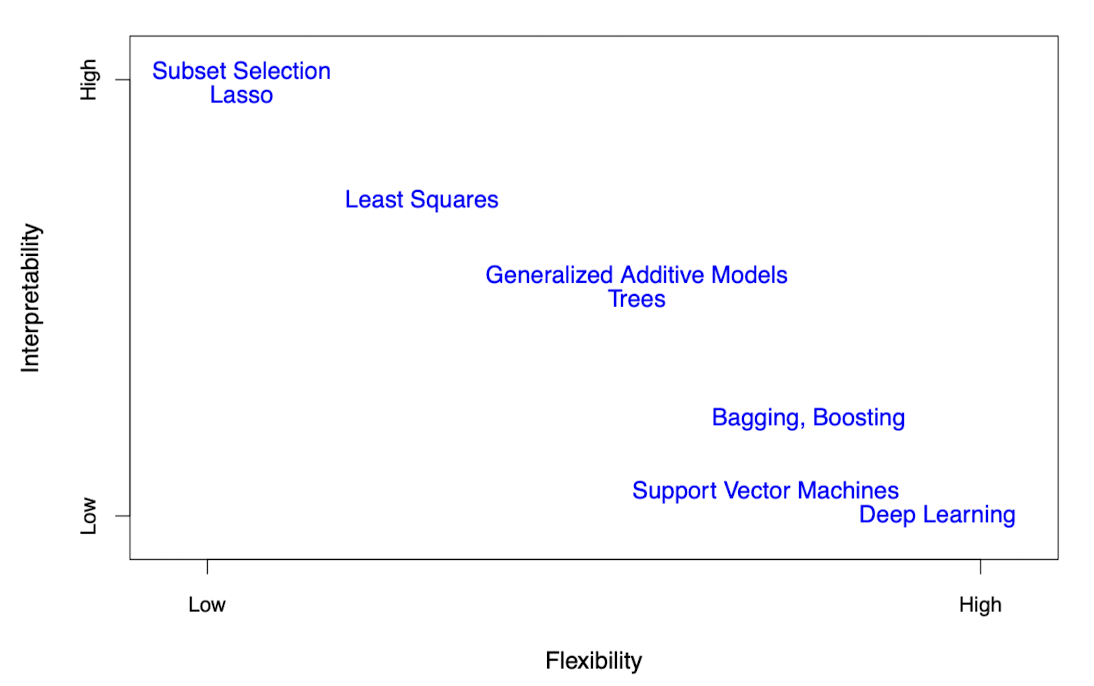
\includegraphics[width=0.7\textwidth]{./figures/intro/flexintertradeoff.png}
    \caption{Trade-off between prediction accuracy and model interpretability.}
    \label{fig:flexintertradeoff}
\end{figure}

\subsection*{Supervised and Unsuperivised Learning}
In the context of statistical learning, we can distinguish between two main types of learning: \textbf{supervised} and \textbf{unsupervised} learning.

\subsubsection*{Supervised Learning}
Assume we have a set of observations $(x_i, y_i)$ where $y_i = f(x_i)$ and $x_i = (x_{i1}, \dots, x_{ip})$. The goal is to find a model that explains the relationship between the response variable and the predictions, either for prediction or inference. The learning algorithm is trained on the set of observations and it learns the relationship between the predictors and the response. Examples of supervised learning methods are linear regression, logistic regression, GAM, boosting and SVM,

\subsubsection*{Unsupervised Learning}
For each observation $i=1,\dots,N$, we have a vector of predictors $x_i = (x_{i1}, \dots, x_{ip})$ but we do not have a response variable. In this case, we would like to find a model that explains the relationship between the observations. The most common unsupervised learning method is cluster analysis, which groups observations into clusters based on their similarity.

\subsection*{Model Selection and Assessment}
The \textbf{No-Free-Lunch Theorem} states that no single model is the best for all problems. On some data, a specific model may perform better than others, but on different data, the same model may perform worse. This is why we need to compare different models while training the learning algorithm.

To measure the \textbf{quality} of fit of a model, we need to find a way to measure how much the predicted values differ from the true values. The most common measure is the \textbf{mean squared error} (MSE), which is the average of the squared differences between the predicted values and the true values. If the MSE is low, then the model is a good fit to the data, while if the MSE is high, then the model is a poor fit to the data.

Assume we have a set of observations $\mathcal{D}_{\text{train}} = \{(x_i, y_i)\}$, $i=1,\dots,N$. We can compute the \textbf{training MSE} as follows:
\[
    \text{MSE}_{\text{train}} = \frac{1}{N} \sum_{i=1}^{N} (y_i - \hat{f}(x_i))^2
\]

The training MSE is not a good measure of the fit of the model to the data, because it is computed on the same data that was used to train the model. When we compare models, we are interested in how well they can predict the response given new data. We then need to compute the \textbf{test MSE}. Given a new set of observations $\mathcal{D}_{\text{test}} = \{(x_i, y_i)\}$, $i=1,\dots,N$, we can compute the test MSE as follows:
\[
    \text{MSE}_{\text{test}} = \frac{1}{N} \sum_{i=1}^{N} (y_i - \hat{f}(x_i))^2  
\]

In general, the more flexible the model, the lower the training MSE, because the model can fit the data more closely. Given different models, we can compare them by computing the test MSE. The model with the lowest test MSE is the best model.

\subsection*{Bias-Variance Trade-Off}
Assume we have a fit $\hat{f}(x)$ on a certain training set $\mathcal{D}_{\text{train}}$ and we have a new observation $(x_0, y_0)$. If the true model is $Y = f(X) + \epsilon$ with $\E{}{\epsilon} = 0$, we will have that the \textbf{expected MSE} of the prediction $\hat{f}(x_0)$ is:
\[
    \mathbb{E}[y_0-\hat f(x_0)]^2=\underbrace{[Bias(\hat f(x_0))]^2+Var(\hat f(x_0))}_{\text{Reducible}}+\underbrace{Var(\epsilon)}_{\text{Irreducible}}
\]
where $Bias(\hat f(x_0)) = \mathbb{E}[\hat f(x_0)] - f(x_0)$ is the bias of the estimator and $Var(\hat f(x_0)) = \mathbb{E}[\hat f(x_0)^2] - \mathbb{E}[\hat f(x_0)]^2$ is the variance of the estimator.

We have a \textbf{trade-off} between the bias and the variance of the estimator, because if we increase the flexibility of the model, we will decrease the bias but increase the variance. 

The \textbf{bias} of the estimator is the error that is introduced by approximating a real-life problem, which may be extremely complicated, by a much simpler model. We can decrease the bias by using more complex and flexible models. The \textbf{variance} of the estimator expresses how much the estimate of the target function will change if different training data is used. The more flexible the model, the more variance it will have. If a model has high variance, it will be very sensitive to the training data. 

To minimize the expected test MSE, we need to find the right balance between bias and variance. This is called the \textbf{bias-variance trade-off}. This trade-off is a fundamental concept in statistical learning and it common to all learning algorithms.

\begin{figure}[H]
    \centering
    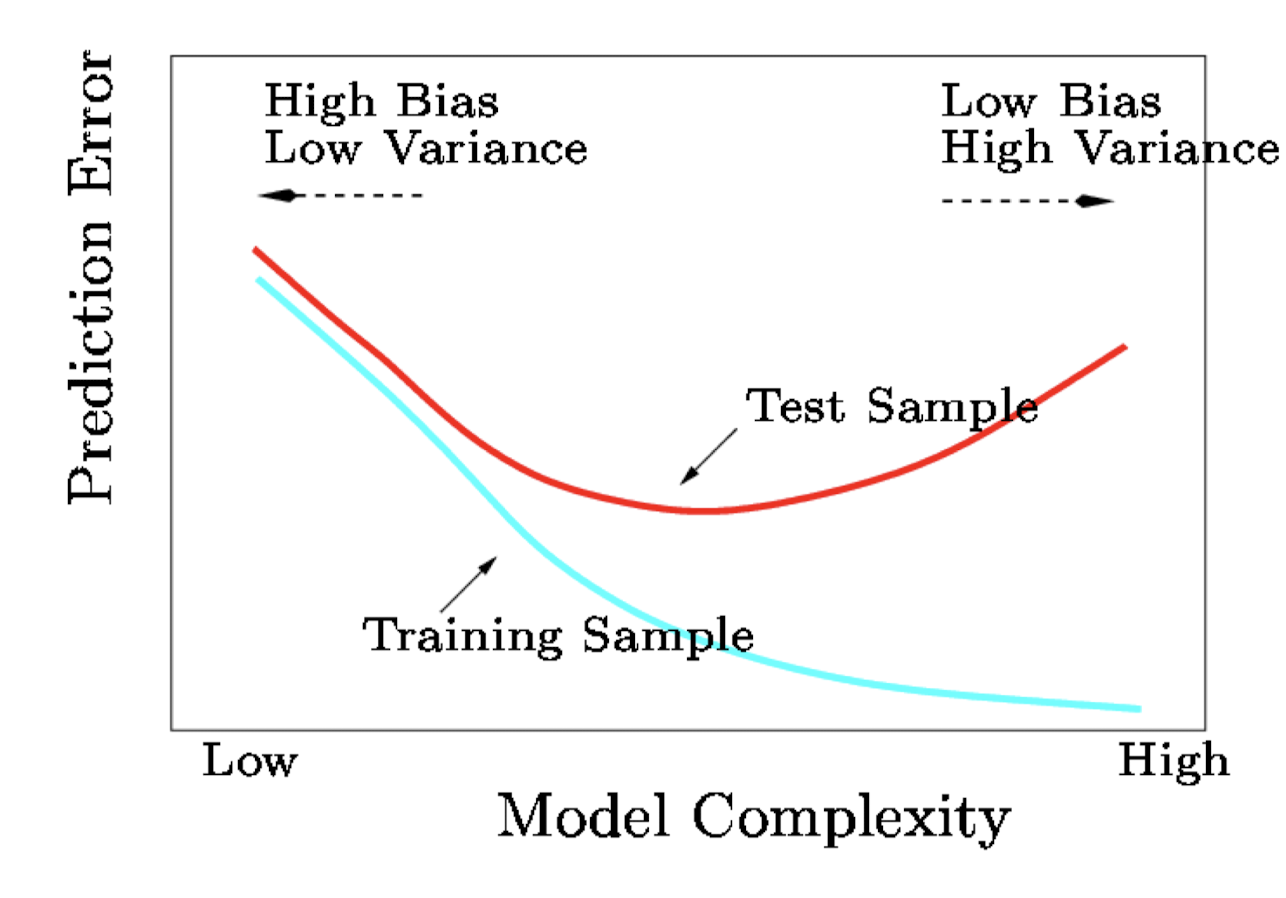
\includegraphics[width=0.7\textwidth]{./figures/intro/biasvariancetradeoff.png}
    \caption{Bias-variance trade-off.}
    \label{fig:biasvariancetradeoff}
\end{figure}

Let us consider some examples of model fitting with different levels of flexibility. In figure \ref*{fig:flexibilitycomparison}, we have three different models: a linear model, a non-linear model, and a non-linear model with high flexibility. 

We can see that when increasing the flexibility of the model, there's a decrease in the training MSE and an \textbf{U-Shape Test MSE}. This is a property that is common to all learning algorithms and datasets. Increasing flexibility implies a decrease in the training MSE but not necessarily in the test MSE. If the test MSE increases, it means that the model is overfitting the data.

Estimating the test MSE is not easy because there are not enough data to compute an accurate estimate. There are different methods to estimate the test MSE, such as the validation set approach, the cross-validation approach, and the bootstrap approach.

\begin{figure}
    \centering
    \begin{minipage}[b]{0.7\textwidth}
        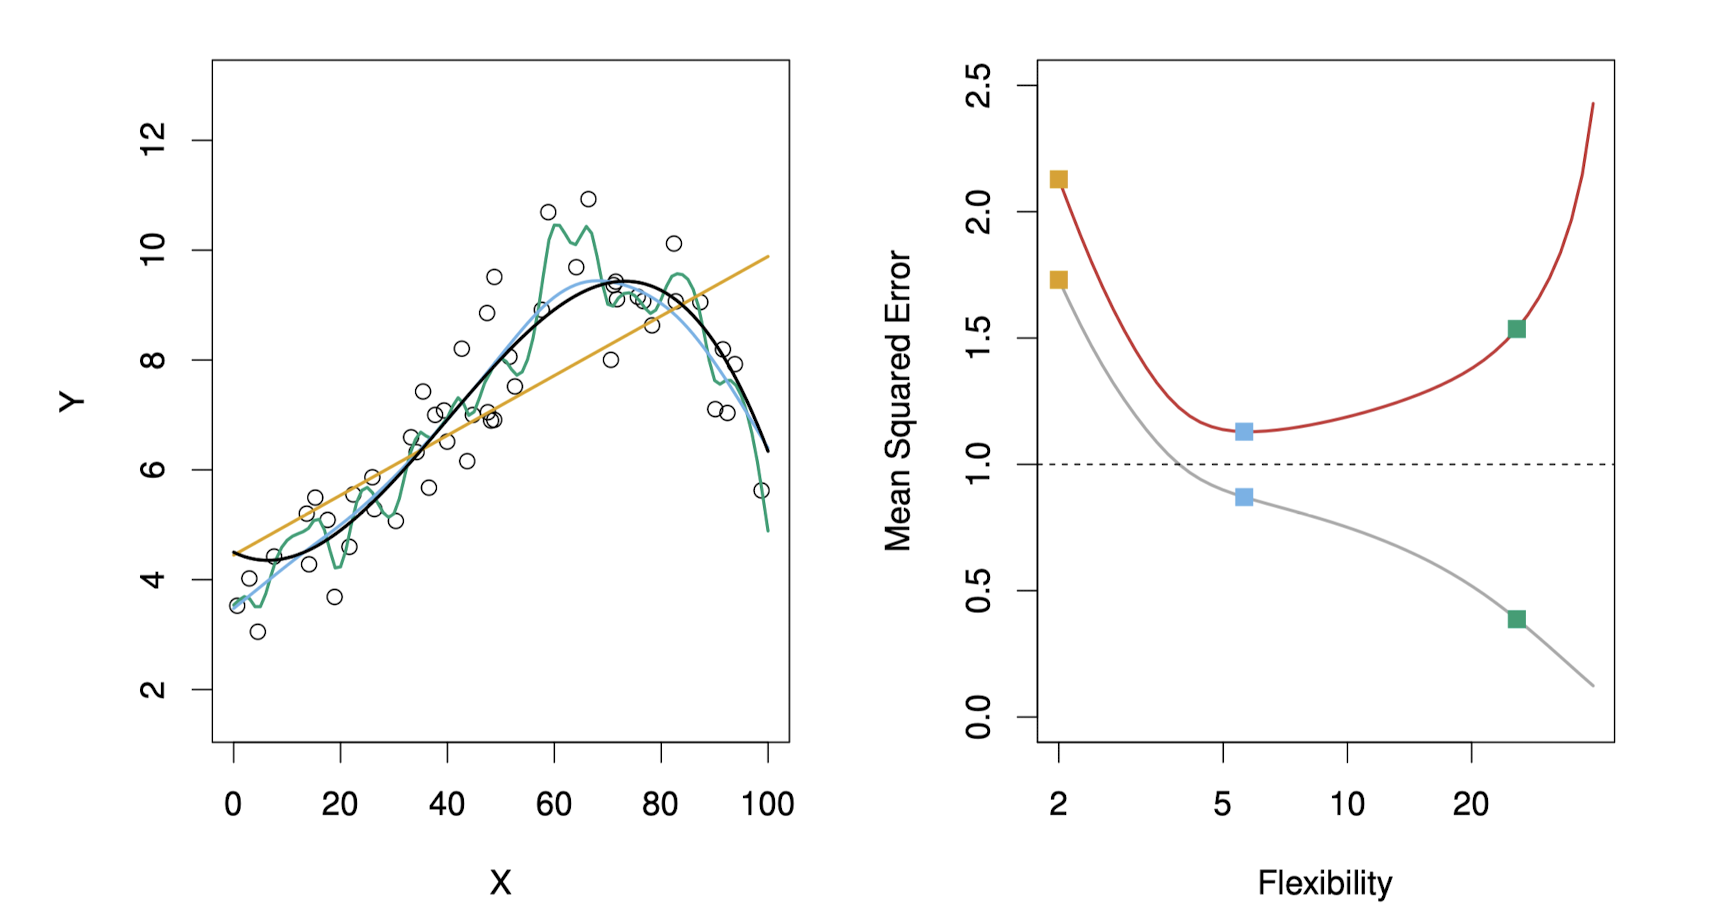
\includegraphics[width=\textwidth]{./figures/intro/flexibilityexample1.png}
    \end{minipage}
    \begin{minipage}[b]{0.7\textwidth}
        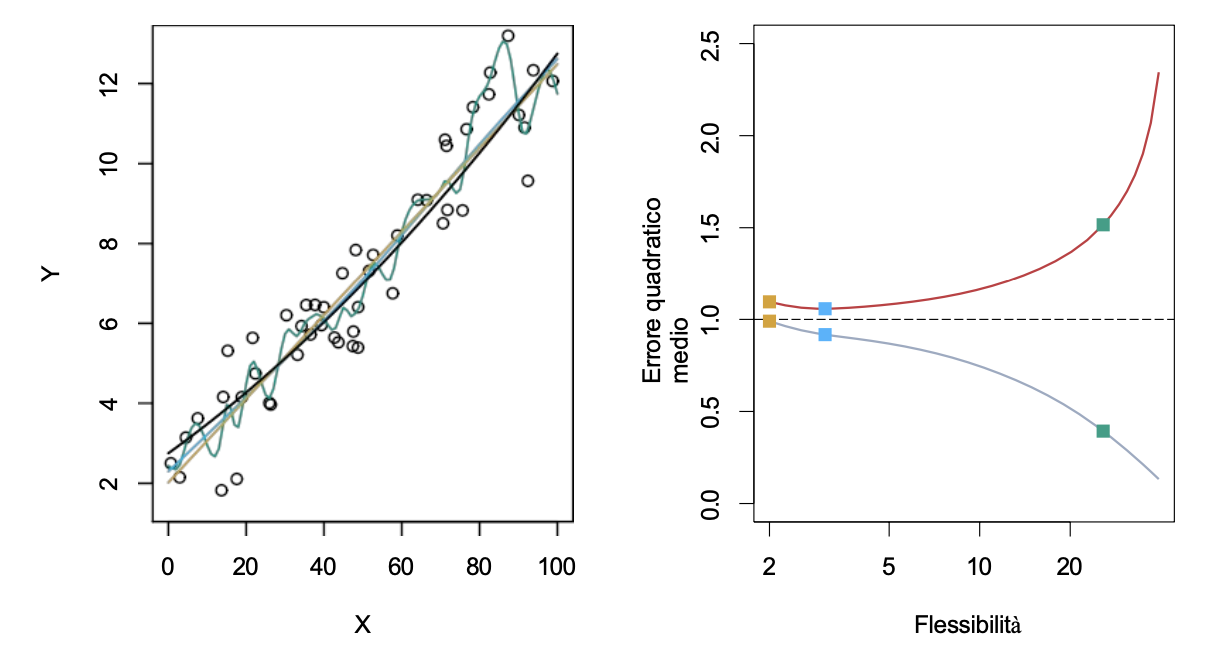
\includegraphics[width=\textwidth]{./figures/intro/flexibilityexample2.png}
    \end{minipage}
    \begin{minipage}[b]{0.7\textwidth}
        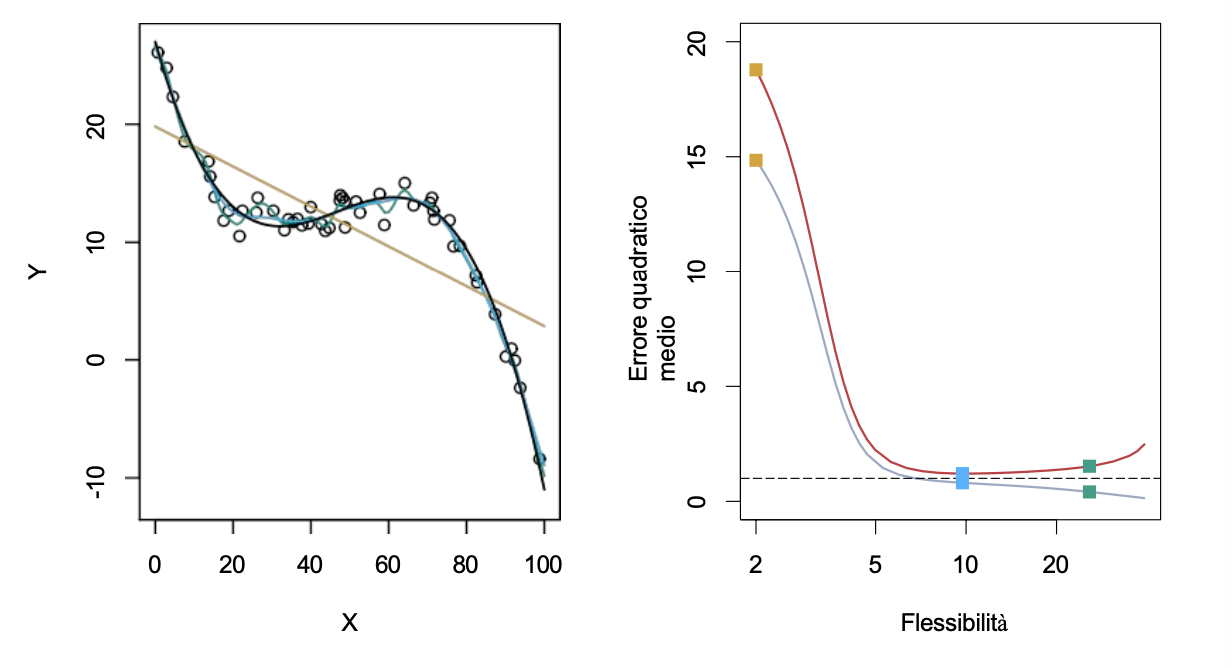
\includegraphics[width=\textwidth]{./figures/intro/flexibilityexample3.png}
    \end{minipage}
    \caption{Comparison of regression models with different levels of flexibility. The plots on the left show the data and the fitted regression function for three different models. The second pictures show the training (red curve) and test (grey curve) MSE for the three models. The dashed linear curve represents the irreducible error. The black curve represents the true regression function. The yellow curve represents a linear estimation, the blue curve represents non-linear estimation and the green curve represents a non-linear estimation with high flexibility.}
    \label{fig:flexibilitycomparison}
\end{figure}

\begin{figure}[H]
    \centering
    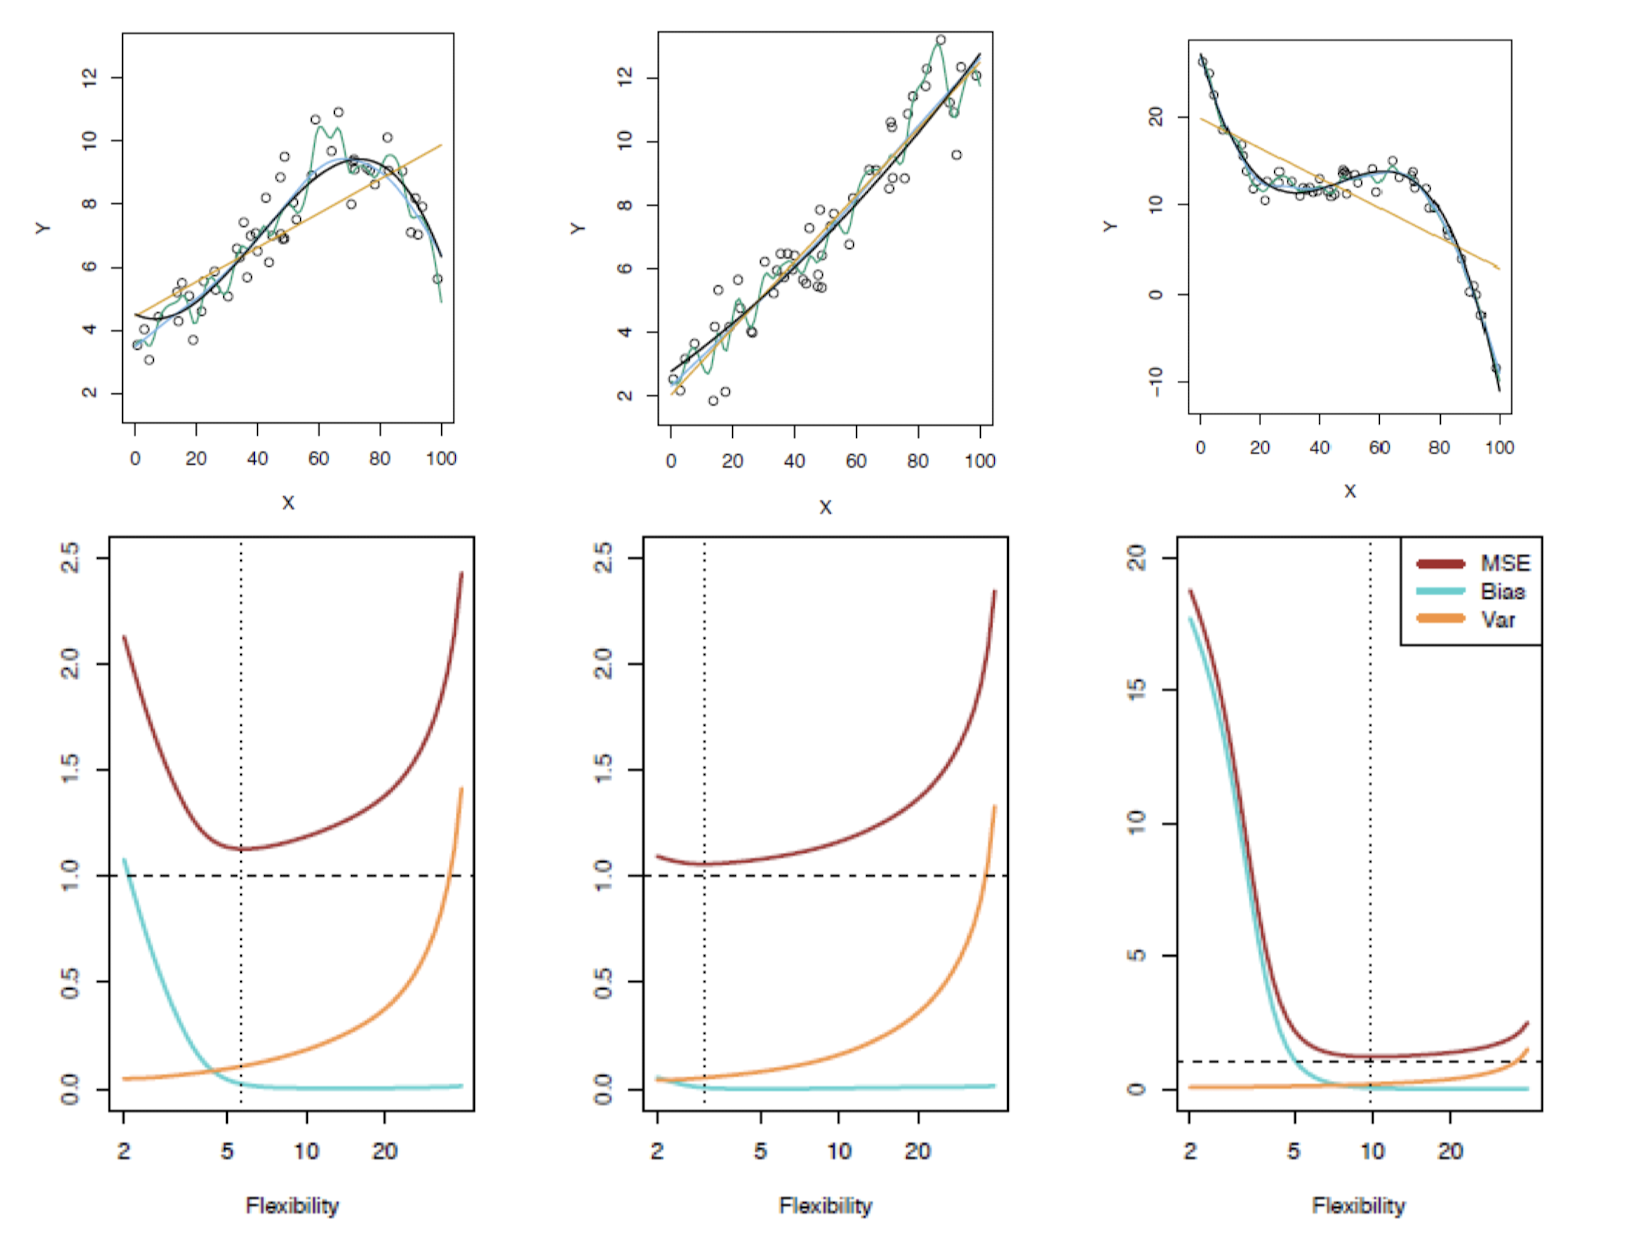
\includegraphics[width=0.7\textwidth]{./figures/intro/flexibilityexample4.png}
    \caption{Bias-variance trade-off for three different models.}
    \label{fig:flexibilityexample4}
\end{figure}

The three plots above shows the expected test MSE for the three models. The blue curve represents the (squared) bias term for different levels of flexibility, while the organe curve represents the variance term. The dashed line represents the irreducible error and the red curve represents the expected test MSE, which is the sum of all three of them. 

In all of the examples, the variance increases with the flexibility of the model, while the bias decreases. The flexibility level that minimizes the expected test MSE differs for each model, because the bias and variance trade-off is different for each model.

\newpage
\section*{Data Analysis}
Data Analysis is the process of extracting information from data. Although data and information are often used interchangeably, they are not the same. Data is something that should cointain information, but it is not information itself. In order to extract information from data, we need to build a learning system.

An important thing to know is that when the learning system is \textit{good}, then by increasing the amount of data we have, the available information cannot decrease. In practice, most of the times we do not have a good system (due to analytical, computational, or time skills not available), so it can happen that the data fed to the system is misleading and the information we get from the analysis decreases. A \textit{non optimal} system could be attacked using fake data in order to decrase information and make the system less reliable; the \textit{optimal} system is able to discard that data.

The two main families of problems in data analysis are \textit{estimation} and \textit{classification}. The main difference is that in the estimation problem,
we have a set of data and we want to estimate a real value, while in the classification problem the output is contained in a finite set. This difference is projected onto the output response variable $Y$.

\begin{figure}[H]
    \centering
    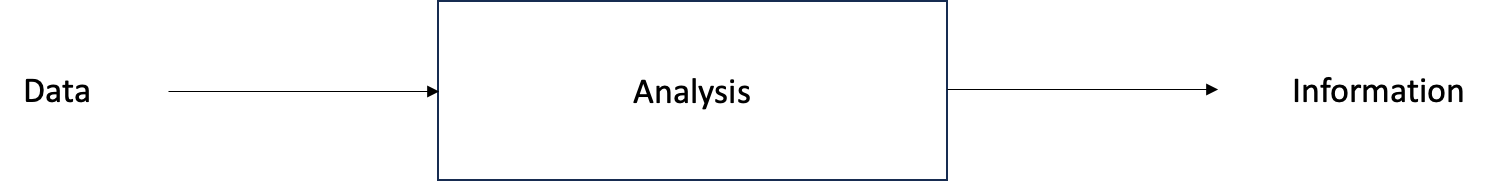
\includegraphics[width=0.7\textwidth]{./figures/chapter_2/data2information.png}
    \caption{The general process of extracting information from data.}
    \label{fig:data2information}
\end{figure}

The input of the learning system can be anything (a vector, a matrix, a graph, a sequence, etc.), but the output is always a real number or a finite set of values. In general,
we do not care about the dimension of the output, because we can always repeat the problem as many times as the dimension of the output.

% qualcosa sul fatto che esiste model based analysis e supervised parametric e non parametric

Data analysis problems don't necessary require a \textit{training phase}. We can have two scenarios:
\begin{enumerate}
    \item \textbf{Model-Based}, the model is given to us.

          \begin{figure}[H]
              \centering
              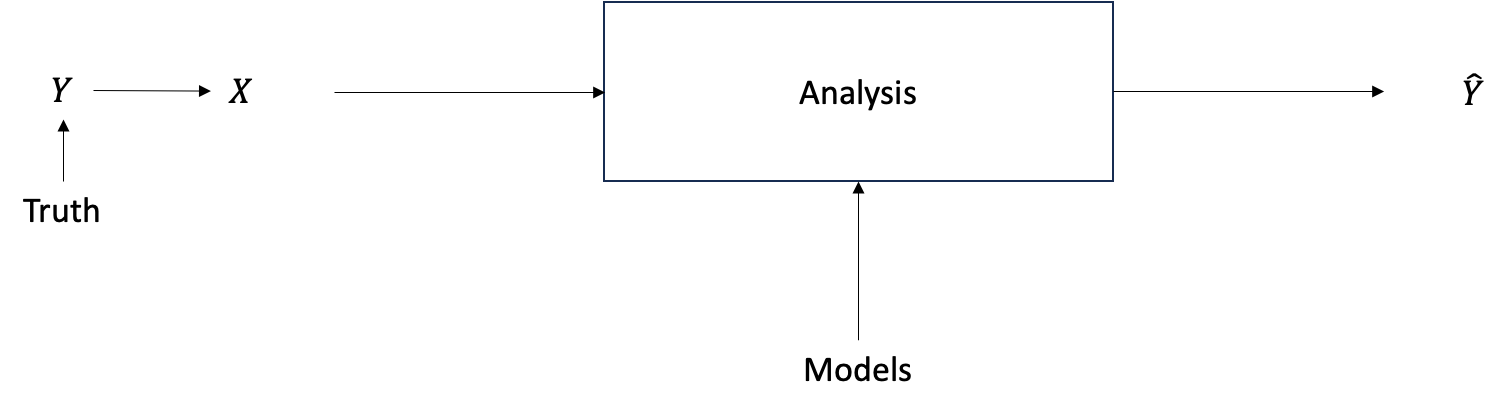
\includegraphics[width=0.7\textwidth]{./figures/chapter_2/modelbased.png}
              \caption{The model based process of extracting information from data.}
              \label{fig:modelbased}
          \end{figure}

          Figure \ref{fig:modelbased} show the scenario. The truth $Y$ influences the data $X$, hidden in it.

          \callout{Note}{Another thing to make clear is that in statistical learning, we do not have a temporal correlation between the variables. When we say that two variables depend on each other, we just mean that they are correlated, without implying the causality.}

    \item \textbf{Model Learning}, we have to learn a statistical characterization of the couple $(X,Y)$.

          \begin{figure}[H]
              \centering
              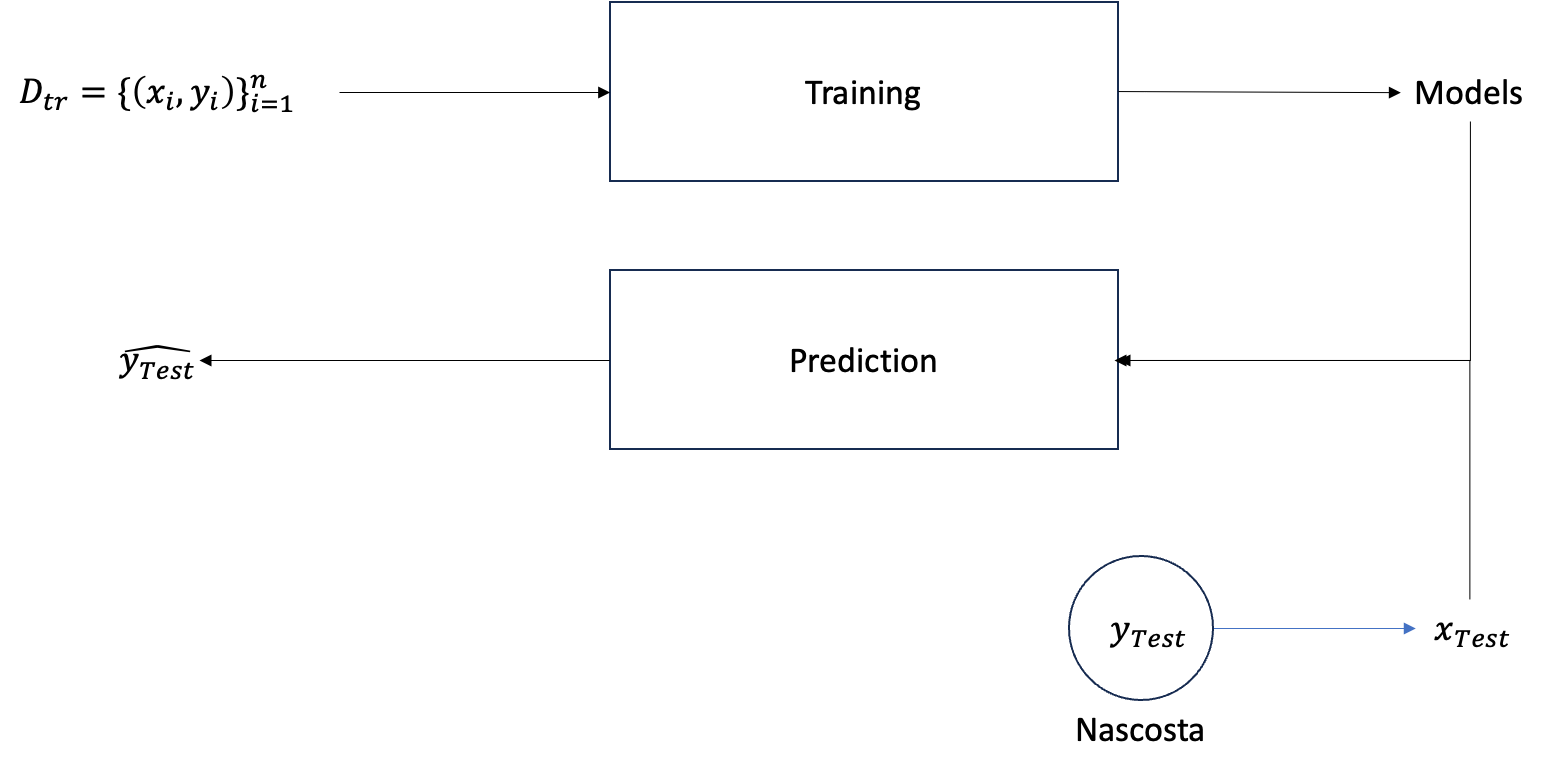
\includegraphics[width=0.7\textwidth]{./figures/chapter_2/modellearning.png}
              \caption{The model learning process of extracting information from data.}
              \label{fig:modellearning}
          \end{figure}

          This scenario could be seen as a \textit{supervised learning} problem when we starts from a set of examples $\mathcal{D}$ to learn the model.
          \[
              \mathcal{D} = \left\{ x_i, y_i \right\}_{i=1}^{N}
          \]
          Figure \ref{fig:modellearning} explain this scenario.


\end{enumerate}
